% Parkin' Space – ITSD 85 Lab 5 paper (IEEE conference format).
% Build on Overleaf: New Project -> Upload Project (this file + the screenshots it uses),
% compiler pdfLaTeX. IEEEtran.cls is built into Overleaf.
% Everything that waits for the playtest is marked \DATA{...} and prints in red,
% so nothing can be submitted with a blank still in it. Search for "\DATA" before submitting.
\documentclass[conference]{IEEEtran}
\usepackage{cite}
\usepackage{amsmath}
\usepackage{graphicx}
\usepackage{booktabs}
\usepackage{xcolor}
\usepackage{listings}
\usepackage{tikz}
\usetikzlibrary{arrows.meta,positioning,fit,shapes.geometric}
\usepackage{url}

\newcommand{\DATA}[1]{\textcolor{red}{\textbf{[DATA: #1]}}}
\newcommand{\game}{\textit{Parkin' Space}}

\lstdefinelanguage{GDScript}{
  morekeywords={func,var,const,if,elif,else,return,for,in,and,or,not,extends,class_name,void,bool,int,float,true,false},
  sensitive=true, morecomment=[l]{\#}, morestring=[b]"}
\lstset{language=GDScript, basicstyle=\ttfamily\scriptsize, keywordstyle=\bfseries,
  commentstyle=\itshape, columns=fullflexible, frame=single, numbers=left,
  numberstyle=\tiny, xleftmargin=1.5em, framexleftmargin=1.5em, tabsize=4}

\begin{document}

\title{Design and Player Evaluation of \game: A Physics-Based Mobile Parking Game with Level Progression and Host-Authoritative Online Multiplayer Built with Open-Source Tools}

\author{\IEEEauthorblockN{Ethan Campomanes}
\IEEEauthorblockA{\textit{BSIT 4C, College of Information Sciences and Computing}\\
\textit{Central Mindanao University}\\
Musuan, Bukidnon, Philippines\\
\DATA{school email}}}

\maketitle

\begin{abstract}
Casual mobile games often trade depth for simplicity, and student projects that add online play usually depend on servers they cannot afford to run. This paper reports the design, implementation and player evaluation of \game, a top-down zero-gravity valet-parking game for Android in which every ship is a rigid body pushed by thrusters drawn on its hull, so that each ship handles differently. The game was built in five weeks by one developer at zero cost with Godot~4.7 and GDScript. It offers a step-by-step tutorial, five levels that each add one new mechanic and unlock in order, an offline campaign, and a same-Wi-Fi one-versus-one duel in which the host phone runs the only simulation and decides the winner. \DATA{n} participants from outside the team played Levels 1--3 and one online match while thinking aloud, then rated the game on a 15-item, five-point Likert form. \DATA{overall M and SD; strongest and weakest items with M; completion rate of Levels 1--3}. Playtest feedback led to \DATA{number} changes, including a guided tutorial for players who skipped the written guide, and a retest with \DATA{n} new participants showed \DATA{retest outcome}. The results suggest that \DATA{one-sentence conclusion}.
\end{abstract}

\begin{IEEEkeywords}
mobile game, level design, physics-based gameplay, multiplayer networking, playtesting, Godot
\end{IEEEkeywords}

%=====================================================================
\section{Introduction}
Precision and physics games, from lunar landers to car-parking puzzles, have stayed popular on phones because a single, simple goal can still demand skill. \game\ moves the familiar parking task into zero gravity: nothing slows a ship except the pilot, so every input must later be cancelled by another one. Players work as valets in dark space parking lots, collecting ships from an arrivals bay, parking them in spaces of the right size class, and returning them to an exit pad when their owners come back, while any hard collision is deducted from their pay.

The project was built under the constraints of a course laboratory: one developer, five weeks, free and open-source tools only, and a required feature set of at least five levels with locked progression, an offline mode that works in airplane mode, and a real-time online mode between two phones. These constraints raise three questions that guided the evaluation:
\begin{itemize}
\item \textbf{RQ1:} Does the level-unlocking system motivate players to continue playing?
\item \textbf{RQ2:} How usable are the offline and online modes on a real phone?
\item \textbf{RQ3:} Which design changes did playtest feedback lead to, and did they improve the retest results?
\end{itemize}

This paper makes three contributions. First, it describes a \emph{thruster-marker pipeline} in which an artist paints thruster positions beside a ship's sprite and the handling follows automatically within a per-class force budget. Second, it describes a host-authoritative LAN duel for a physics game, built only on Godot's built-in ENet transport without a dedicated server. Third, it reports a playtest with \DATA{n} participants and the design changes it produced.

%=====================================================================
\section{Related Work}
\subsection{Motivation, challenge and difficulty}
Self-determination theory explains game enjoyment through the satisfaction of competence, autonomy and relatedness needs~\cite{ryan2006}, and the recent Basic Needs in Games Scale measures both the satisfaction and the frustration of these needs~\cite{ballou2024}. Flow theory adds that engagement peaks when challenge matches skill~\cite{csikszentmihalyi1990}. Studies of difficulty pacing found that the way difficulty rises across a game affects player motivation~\cite{raofernandes2022}, while dynamic difficulty adjustment changes challenge at run time to keep it in balance~\cite{robb2022}. \game\ takes the simpler, fixed route recommended for short campaigns: hand-made levels that each introduce exactly one new element, with the difficulty setting changing only the shift length.

\subsection{Touch controls on phones}
On-screen controls lack the tactile feedback of physical buttons, and comparisons of virtual gamepad layouts showed that their design strongly affects performance and user experience~\cite{baldauf2015}. \game\ responds with large hexagonal buttons, brakes that cancel motion automatically while held (STOP and Stop Spin), a separate lot view in which ships are chosen by tapping them, and, after playtesting, a guided tutorial.

\subsection{Online multiplayer and latency}
Client--server games hide network delay with techniques such as interpolation, prediction and lag compensation~\cite{bernier2001}, which a recent survey organizes into a taxonomy of latency-compensation methods~\cite{liu2022}. For networked physics, a common choice is to let one machine simulate and the others interpolate its state~\cite{fiedler2015}. Godot exposes this model through its high-level multiplayer API over ENet~\cite{godotdocs}, and the engine's growing role in independent development has been documented~\cite{holfeld2023}. \game\ uses entity interpolation without client-side prediction, a trade-off that is acceptable on a local network.

\subsection{Playtesting methods}
Games user research combines observation, think-aloud sessions and questionnaires~\cite{desurvire2013,drachen2018}. The ``play aloud'' variant borrows from game-commentary culture to make thinking aloud more natural~\cite{pellicone2022}. Likert items in this study are reported as means and standard deviations, following common guidance for analyzing Likert data~\cite{boone2012}.

%=====================================================================
\section{Game Design}
\subsection{Core loop, goal, and win and lose rules}
Ships arrive in the ARRIVALS bay, which pulses while a ship is waiting. The player taps a ship to take control, drives it with thrusters into a space of its class (light, medium or heavy) or larger, waits for the space to turn orange, and presses Done to park. Later, owners ask for their ships back, and the player drives them onto the EXIT pad. Each shift starts with a base salary. Hard impacts above a safe speed of 120~px/s cost pay, while park fees and tips add to earnings. A level is \emph{won} when every customer has been served before the shift ends. It is \emph{lost} when pay reaches zero (``You're fired!'') or when the shift ends with customers still waiting. Stars (one to three) are awarded by comparing earnings with each level's silver and gold targets. A thin glow at the screen edges, green at rest, yellow at the safe speed and red at 600~px/s, warns the player while driving how costly a crash would be.

\subsection{Ships}
The game contains ten original ships in three classes (four light, three medium and three heavy). Because handling is derived from where thrusters are drawn (Section~\ref{sec:impl}), ships of the same class still feel different, for example a nose-heavy drone or a saucer that spins easily.

\subsection{Levels and progression}
Table~\ref{tab:levels} lists the level plan. A tutorial lot comes first. It cannot be failed and teaches the controls in twelve steps, each waiting until the player has done it. A pulsing ring and an arrow mark whatever must be tapped. It opens automatically the first time the player chooses Offline and stays available on the level-select screen. Clearing level $n$ unlocks level $n+1$, and the shift length is set by the chosen difficulty (Easy 10:00, Normal 5:00, Hard 2:30).

\begin{table}[t]
\caption{Level Plan}
\label{tab:levels}
\centering
\footnotesize
\begin{tabular}{@{}p{0.9cm}p{1.9cm}p{4.6cm}@{}}
\toprule
Level & Goal on screen & New or harder element \\
\midrule
Tutorial & Twelve guided steps & Selecting, Done, driving, stopping in a space, spin control, EXIT; cannot be failed \\
1 Starter & Park 4 ships & Light and medium ships; three lane angles; on-screen hints \\
2 Blossom & Serve 6 customers & Heavy ships; tip tiers; retrieval requests and the EXIT pad \\
3 Wreckage & Serve 7 customers & Fixed wrecks, drifting asteroids, radiation zones that dent ships \\
4 Gravity Well & Serve 7 customers & A black hole that pulls and flings ships and asteroids; orphaned ships to eject \\
5 Gold Lounge & Serve 9 customers & 60\% gold customers, special space requests, movable parked ships, pillars and a walled-off exit \\
\bottomrule
\end{tabular}
\end{table}

\subsection{Offline and online modes}
The offline mode is the solo campaign and needs no network at all. The online mode is a one-versus-one duel on a symmetric lot between two phones on the same Wi-Fi. Two seeded arrival bays hand both players ships of the same class and tip tier in matching order. Every ship leaves 20--30~s after it is first parked: the fee goes to whoever parked it, and the tip to whoever delivers it to the EXIT. Dent costs follow the last player who controlled a ship, and when two driven ships collide the faster one pays. The host picks a match length of 3--20 minutes. Online results do not affect offline unlocking. Fig.~\ref{fig:flow} shows the screen flow, including the connection-error path.

\begin{figure}[t]
\centering
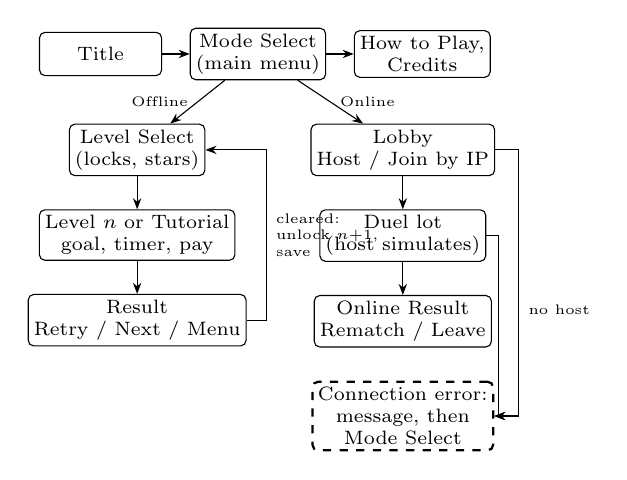
\begin{tikzpicture}[
  scr/.style={draw, rounded corners=2pt, font=\scriptsize, align=center, minimum height=0.55cm, minimum width=1.55cm, inner sep=2pt},
  err/.style={scr, dashed, thick},
  >={Stealth[length=4pt]}, node distance=0.42cm and 0.35cm]
\node[scr] (title) {Title};
\node[scr, right=of title] (mode) {Mode Select\\(main menu)};
\node[scr, right=of mode] (extra) {How to Play,\\Credits};
\node[scr, below left=0.55cm and -0.2cm of mode] (ls) {Level Select\\(locks, stars)};
\node[scr, below right=0.55cm and -0.2cm of mode] (lobby) {Lobby\\Host / Join by IP};
\node[scr, below=of ls] (lvl) {Level $n$ or Tutorial\\goal, timer, pay};
\node[scr, below=of lvl] (res) {Result\\Retry / Next / Menu};
\node[scr, below=of lobby] (duel) {Duel lot\\(host simulates)};
\node[scr, below=of duel] (ores) {Online Result\\Rematch / Leave};
\node[err, below=of ores] (nerr) {Connection error:\\message, then\\Mode Select};
\draw[->] (title) -- (mode);
\draw[->] (mode) -- (extra);
\draw[->] (mode) -- node[left, font=\tiny] {Offline} (ls);
\draw[->] (mode) -- node[right, font=\tiny] {Online} (lobby);
\draw[->] (ls) -- (lvl);
\draw[->] (lvl) -- (res);
\draw[->] (res.east) -- ++(0.25,0) |- node[pos=0.25, right, font=\tiny, align=left] {cleared:\\unlock $n{+}1$,\\save} (ls.east);
\draw[->] (lobby) -- (duel);
\draw[->] (duel) -- (ores);
\draw[->] (lobby.east) -- ++(0.3,0) |- node[pos=0.3, right, font=\tiny] {no host} (nerr.east);
\draw[->] (duel.east) -- ++(0.15,0) |- (nerr.east);
\end{tikzpicture}
\caption{Screen flow. The first Offline tap opens the Tutorial; levels unlock in order and save before the result screen; every level and the duel have a pause menu; any online failure ends on a message and returns to Mode Select.}
\label{fig:flow}
\end{figure}

%=====================================================================
\section{Implementation}
\label{sec:impl}
\subsection{Tools and structure}
The game was built with Godot~4.7.2 (MIT license) in statically typed GDScript, using the Compatibility renderer for older phones and a fixed landscape orientation. Code was versioned with Git on GitHub, and Android builds were exported with OpenJDK~17 and the Android SDK command-line tools. Ship art was drawn by the developer; sound effects come from Kenney (CC0), music from ccMixter (CC~BY-NC~3.0), and the interface font is Orbitron (SIL Open Font License).

The project contains about 7,500 lines of GDScript in 57 game scripts (Fig.~\ref{fig:arch}). Three autoloads hold global services: \texttt{GameState} (progress and settings), \texttt{Sound} and \texttt{Net} (the network session). Every level scene uses one shared \texttt{Level} script, configured in the editor; \texttt{DuelLevel} and \texttt{TutorialLevel} extend it. Gameplay rules live in small, separately tested classes, among them \texttt{ShiftLedger} (pay, tips, dents and outcome), \texttt{ParkingRules}, \texttt{Customer} and \texttt{ShipPilot}, whose \texttt{LocalPilot} and \texttt{NetPilot} variants drive a ship from the touch pad or from the network. A headless test runner executes 495 automated tests in 37 test files before every merge.

\begin{figure}[t]
\centering
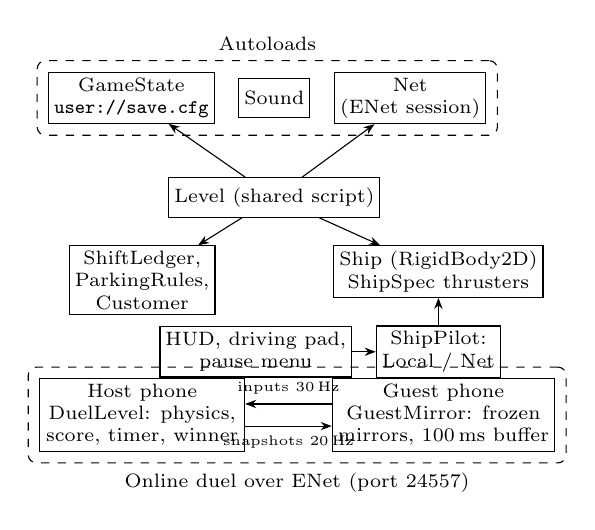
\begin{tikzpicture}[
  box/.style={draw, font=\scriptsize, align=center, minimum height=0.5cm, inner sep=2pt},
  grp/.style={draw, dashed, rounded corners=3pt, inner sep=4pt},
  >={Stealth[length=4pt]}, node distance=0.3cm and 0.3cm]
\node[box] (gs) {GameState\\\texttt{user://save.cfg}};
\node[box, right=of gs] (snd) {Sound};
\node[box, right=of snd] (net) {Net\\(ENet session)};
\node[grp, fit=(gs)(snd)(net), label={[font=\scriptsize]above:Autoloads}] (auto) {};
\node[box, below=0.75cm of snd, minimum width=2.4cm] (lvl) {Level (shared script)};
\node[box, below left=0.35cm and -0.6cm of lvl] (rules) {ShiftLedger,\\ParkingRules,\\Customer};
\node[box, below right=0.35cm and -0.6cm of lvl] (ship) {Ship (RigidBody2D)\\ShipSpec thrusters};
\node[box, below=0.35cm of ship] (pilot) {ShipPilot:\\Local / Net};
\node[box, left=0.3cm of pilot] (ui) {HUD, driving pad,\\pause menu};
\draw[->] (lvl) -- (rules);
\draw[->] (lvl) -- (ship);
\draw[->] (pilot) -- (ship);
\draw[->] (ui) -- (pilot);
\draw[->] (lvl) -- (gs);
\draw[->] (lvl) -- (net);
% duel
\node[box, below=0.8cm of rules, minimum width=2.6cm] (host) {Host phone\\DuelLevel: physics,\\score, timer, winner};
\node[box, right=1.1cm of host, minimum width=2.4cm] (guest) {Guest phone\\GuestMirror: frozen\\mirrors, 100\,ms buffer};
\draw[->] ([yshift=4pt]guest.west) -- node[above, font=\tiny] {inputs 30\,Hz} ([yshift=4pt]host.east);
\draw[->] ([yshift=-4pt]host.east) -- node[below, font=\tiny] {snapshots 20\,Hz} ([yshift=-4pt]guest.west);
\node[grp, fit=(host)(guest), label={[font=\scriptsize]below:Online duel over ENet (port 24557)}] {};
\end{tikzpicture}
\caption{Architecture: global autoloads, the shared level script and its components, and the host-authoritative duel.}
\label{fig:arch}
\end{figure}

\subsection{Thruster-marker pipeline}
Each ship's sprite has a companion marker image in which thrusters are painted by color: red for forward, blue for retro, green for sideways, yellow for rotation and magenta for the center of mass. A build tool converts the markers into a \texttt{ShipSpec} resource. Each ship class has a fixed force budget per button, which is shared among that button's thrusters in proportion to their painted pixel counts. A thruster that is off the center of mass therefore produces torque, so a ship's quirks come directly from where its thrusters were drawn, and new ships need no hand-tuned numbers.

\subsection{Saving and unlocking}
Progress is stored with Godot's \texttt{ConfigFile} in \texttt{user://save.cfg}, the app's private storage on the phone. Listing~\ref{lst:save} shows the unlocking rule: a level is open when its number is at most \texttt{unlocked\_level}, and clearing the frontier level raises it and saves at once, so progress survives a force-close.

\begin{lstlisting}[caption={Unlocking and saving (\texttt{autoload/GameState.gd}).}, label={lst:save}, float=t]
func is_unlocked(level: int) -> bool:
	return level <= unlocked_level

func complete_level(level: int, stars: int) -> void:
	best_stars[level] = maxi(stars, best_stars.get(level, 0))
	if level == unlocked_level and level < TOTAL_LEVELS:
		unlocked_level = level + 1
	save_progress()

func save_progress() -> void:
	var cfg := ConfigFile.new()
	cfg.set_value("progress", "unlocked_level", unlocked_level)
	cfg.set_value("progress", "best_stars", best_stars)
	cfg.save(save_path)   # user://save.cfg
\end{lstlisting}

\subsection{Networking and winner authority}
The duel uses \texttt{ENetMultiplayerPeer} on port 24557 between two phones on the same Wi-Fi, with no server. The host is authoritative: it runs all physics, collisions, scoring and the match timer. The guest sends its button states 30 times per second, and the host replies with state snapshots 20 times per second. On the guest, ships are frozen mirrors drawn 100~ms in the past by interpolating between snapshots, which hides jitter at the cost of a small, constant delay. A protocol version check runs during the handshake. A watchdog on each phone ends the match if nothing has arrived from the other phone for 3~s (10~s while a scene is loading) and returns the player to Mode Select with a message. The winner is decided only by the host and announced to both phones, so the two phones can never disagree and a modified guest cannot report a false score.

\subsection{Android build}
The game was exported as a debug-signed APK of about 84~MB with the Internet and Access Network State permissions, and installed directly on the test phones. It was tested on a Huawei LYA-L29 (Android~10) and \DATA{second phone model and Android version}; Appendix~C gives the phone test matrix.

%=====================================================================
\section{Evaluation Method}
\subsection{Participants}
\DATA{n} participants from outside the development team took part. Table~\ref{tab:participants} summarizes their age ranges and how often they play mobile games. A further \DATA{n} new participants took part in the retest after the fixes.

\begin{table}[t]
\caption{Participant Profile}
\label{tab:participants}
\centering
\footnotesize
\begin{tabular}{@{}lcc@{}}
\toprule
 & First round & Retest \\
\midrule
Participants ($n$) & \DATA{} & \DATA{} \\
Age under 18 / 18--24 / 25+ & \DATA{} & \DATA{} \\
Play mobile games daily / weekly / rarely & \DATA{} & \DATA{} \\
\bottomrule
\end{tabular}
\end{table}

\subsection{Procedure}
Each session lasted 15--20 minutes on a freshly installed build. Participants received a one-sentence brief, ``Please play as you normally would and say out loud what you are thinking,'' with no explanation of the controls or the goal. They played Levels 1--3 offline on the Normal difficulty and then one three-minute online duel against the developer, joining the developer's phone over the same Wi-Fi. The developer observed silently, helped only after a participant had been stuck for more than two minutes, and recorded every instance of help.

\subsection{Instrument and analysis}
After playing, each participant completed the laboratory's 15-item feedback form on a five-point Likert scale (1~= strongly disagree, 5~= strongly agree) and six open questions. The developer completed an observation sheet that recorded, per level, the attempts, time to clear, points of confusion, quotes and bugs. Each Likert item was summarized by its mean ($M$), standard deviation ($SD$) and $n$, and interpreted with the bands 4.20--5.00 strongly agree, 3.40--4.19 agree, 2.60--3.39 neutral, 1.80--2.59 disagree and 1.00--1.79 strongly disagree; items below 3.5 were treated as problem areas. For each level the completion rate and mean attempts were computed. Open answers were coded into the themes controls, difficulty, clarity, bugs, online, and art and sound.

\subsection{Ethics}
Every participant gave written consent before playing, and participants under 18 also had a parent's or guardian's consent. Participants are identified only by codes (T1, T2, \ldots); no names, faces or phone numbers were collected, in line with the Philippine Data Privacy Act of 2012 (RA~10173). All responses are reported, including negative ones.

%=====================================================================
\section{Results}
\subsection{Questionnaire}
Table~\ref{tab:likert} lists the ratings for all 15 items. \DATA{two or three sentences: highest items, lowest items, any item below 3.5}.

\begin{table}[t]
\caption{Feedback Form Results (5-point scale)}
\label{tab:likert}
\centering
\footnotesize
\begin{tabular}{@{}rp{4.5cm}ccc@{}}
\toprule
\# & Statement & $M$ & $SD$ & $n$ \\
\midrule
1 & The game was fun to play. & \DATA{} & & \\
2 & I understood the goal of each level without help. & \DATA{} & & \\
3 & The touch controls were easy and responsive. & \DATA{} & & \\
4 & Each level felt a little harder than the last, but fair. & \DATA{} & & \\
5 & Unlocking the next level made me want to keep playing. & \DATA{} & & \\
6 & The win/lose result screen clearly showed how I did. & \DATA{} & & \\
7 & Offline mode worked smoothly. & \DATA{} & & \\
8 & Joining an online match was easy. & \DATA{} & & \\
9 & The online match felt responsive (little or no lag). & \DATA{} & & \\
10 & The graphics were clear and attractive. & \DATA{} & & \\
11 & The sound and music fit the game. & \DATA{} & & \\
12 & Text and buttons were easy to read and tap. & \DATA{} & & \\
13 & The game ran without crashes or freezes. & \DATA{} & & \\
14 & I would play this game again. & \DATA{} & & \\
15 & I would recommend this game to a friend. & \DATA{} & & \\
\bottomrule
\end{tabular}
\end{table}

\subsection{Level completion}
Fig.~\ref{fig:completion} shows the completion rate of each level. \DATA{completion rates and mean attempts for Levels 1--3; any level below 60\% or above 4 attempts}.

\begin{figure}[t]
\centering
\fbox{\parbox[c][2.6cm][c]{0.85\columnwidth}{\centering\DATA{bar chart: completion rate (\%) for Levels 1, 2, 3; black and white, made in LibreOffice Calc and saved as \texttt{completion.pdf}}}}
% Replace the box above with: \includegraphics[width=0.9\columnwidth]{completion.pdf}
\caption{Completion rate per level (participants who cleared the level divided by participants who tried it).}
\label{fig:completion}
\end{figure}

\subsection{Themes from open answers}
\DATA{counts per theme, with short quotes tagged by participant code, e.g. ``\ldots'' (T3)}.

\subsection{Changes made and retest}
Table~\ref{tab:actions} lists the issues found and the changes made. The most consequential change was a guided tutorial lot. Playtesters got stuck on the controls and tended to skip the illustrated How to Play guide, so written instructions alone did not work. The tutorial now opens on the first Offline tap and waits at each step until the player has done it, pointing at the exact button to press. \DATA{retest result for each fix}.

\begin{table}[t]
\caption{Action Plan}
\label{tab:actions}
\centering
\footnotesize
\begin{tabular}{@{}p{2.4cm}cp{2.6cm}p{1.2cm}@{}}
\toprule
Issue & Reports & Change & Retest \\
\midrule
Stuck on the controls; guide skipped & \DATA{} & Guided 12-step tutorial; pulsing ARRIVALS bay & \DATA{} \\
No warning before hitting the lot wall & dev. & Red lot-edge glow near walls & \DATA{} \\
Unclear wait while owners are away & dev. & Return countdowns and a HUD waiting line & \DATA{} \\
Thrust buttons held too long & dev. & ``Tap, don't hold'' tip in the guide & \DATA{} \\
Speed hard to judge & dev. & Green--yellow--red speed glow & \DATA{} \\
\bottomrule
\end{tabular}
\end{table}

%=====================================================================
\section{Discussion}
\textbf{RQ1 (motivation from unlocking).} \DATA{items 5 and 14 with M and SD; completion rates; what they say about the one-new-mechanic curve, compared with the difficulty-pacing findings in~\cite{raofernandes2022}}.

\textbf{RQ2 (usability of the offline and online modes).} \DATA{items 3, 7, 8, 9, 12 and 13}. In particular, \DATA{whether item 9 shows that a 100~ms interpolation delay felt responsive on a LAN, compared with the latency-compensation literature~\cite{liu2022}}.

\textbf{RQ3 (effect of playtest-driven changes).} \DATA{whether the retest participants cleared the first steps without help and how the problem items changed}.

\textbf{Limitations.} The sample was small and drawn from fellow students, so the results may not generalize to other players. Only Android was tested, on \DATA{two} phone models. One developer built and evaluated the game, which may bias the observation notes. Online play was tested only on a shared local network, without internet matchmaking. Each session was short, so long-term motivation was not measured.

%=====================================================================
\section{Conclusion and Future Work}
\DATA{main finding in two sentences}. Future work includes internet play through a self-hosted Nakama server, client-side prediction for the guest phone, an accessibility pass with a colour-blind-safe palette for the neon cues, and a larger study across several sessions.

\section*{Acknowledgment}
The author thanks the course instructor, Rinante M. Buntod, and the playtest participants (T1--T\DATA{n}). Claude (Anthropic), used through Claude Code, served as a programming assistant for implementation, automated tests and documentation, and helped draft this paper; the author directed the design, drew the ship art, ran the playtests, and checked and edited all text and code.

%=====================================================================
% References: every entry marked VERIFY must be checked against the publisher page
% (title, authors, venue, volume, pages, year) in Zotero before submission.
\begin{thebibliography}{00}
\bibitem{ryan2006} R. M. Ryan, C. S. Rigby, and A. Przybylski, ``The motivational pull of video games: A self-determination theory approach,'' \textit{Motivation and Emotion}, vol. 30, no. 4, pp. 347--363, 2006.
\bibitem{ballou2024} N. Ballou, A. Denisova, R. M. Ryan, C. S. Rigby, and S. Deterding, ``The Basic Needs in Games Scale (BANGS): A new tool for investigating positive and negative video game experiences,'' \textit{Computers in Human Behavior}, vol. 144, Art. no. 107158, 2023. % VERIFY year and article number
\bibitem{csikszentmihalyi1990} M. Csikszentmihalyi, \textit{Flow: The Psychology of Optimal Experience}. New York, NY, USA: Harper \& Row, 1990.
\bibitem{raofernandes2022} S. Rao Fernandes \textit{et al.}, ``Difficulty pacing impact on player motivation,'' in \textit{Proc. Int. Conf. Entertainment Computing (ICEC)}, 2022. % VERIFY venue, authors, pages (HAL hal-03847459)
\bibitem{robb2022} J. Robb and J. Zhang, ``Performance-based dynamic difficulty adjustment and player experience in a 2D digital game: A controlled experiment,'' \textit{Acta Ludologica}, vol. 5, no. 1, 2022. % VERIFY authors and pages
\bibitem{baldauf2015} M. Baldauf, P. Fr\"ohlich, F. Adegeye, and S. Suette, ``Investigating on-screen gamepad designs for smartphone-controlled video games,'' \textit{ACM Trans. Multimedia Comput., Commun., Appl.}, vol. 12, no. 1s, 2015. % VERIFY
\bibitem{bernier2001} Y. W. Bernier, ``Latency compensating methods in client/server in-game protocol design and optimization,'' in \textit{Proc. Game Developers Conf.}, 2001.
\bibitem{liu2022} S. Liu, X. Xu, and M. Claypool, ``A survey and taxonomy of latency compensation techniques for network computer games,'' \textit{ACM Comput. Surv.}, vol. 54, no. 11s, Art. no. 243, 2022, doi: 10.1145/3519023.
\bibitem{fiedler2015} G. Fiedler, ``Networked physics,'' \textit{Gaffer On Games}, 2014--2015. [Online]. Available: \url{https://gafferongames.com/} % VERIFY exact article title and URL
\bibitem{godotdocs} Godot Engine contributors, ``High-level multiplayer,'' \textit{Godot Engine Documentation} (4.x). [Online]. Available: \url{https://docs.godotengine.org/} % add the page URL and the access date
\bibitem{holfeld2023} C. Holfeld, ``On the relevance of the Godot Engine in the indie game development industry,'' arXiv:2401.01909, 2023. % VERIFY year
\bibitem{desurvire2013} H. Desurvire and M. Seif El-Nasr, ``Methods for game user research: Studying player behavior to enhance game design,'' \textit{IEEE Comput. Graph. Appl.}, vol. 33, no. 4, pp. 82--87, 2013.
\bibitem{drachen2018} A. Drachen, P. Mirza-Babaei, and L. Nacke, Eds., \textit{Games User Research}. Oxford, U.K.: Oxford Univ. Press, 2018.
\bibitem{pellicone2022} B. Pellicone \textit{et al.}, ``Playing aloud: Leveraging game commentary culture for playtesting,'' 2022. % VERIFY journal, volume, authors (IGI Global article 296705)
\bibitem{boone2012} H. N. Boone and D. A. Boone, ``Analyzing Likert data,'' \textit{J. Extension}, vol. 50, no. 2, 2012.
\end{thebibliography}

\end{document}
